\section{Additional SNLI test-set}\label{sec:additional_snli_set}
In the previous section we have identified several lexical inferences, that have not been captured by the model and thus mispredicted.  However we could only consider a small subset of misclassified samples, since a small lexical overlap would result in multiple interpretations of what the model understands and what not. In fact, even when identifying missing knowledge in our anaysis, we needed to rely on intuition rather than certainity when assigning mislabelled samples into categories. We also take a look about what the model seemingly knows, based on its correct predictions, shown in Table \ref{table:correct_samples}.
\begin{table}[!htbp]
\begin{center}
\begin{tabular}{lc}
\textbf{Premise/Hypothesis} & \textbf{Label} \\
\toprule
\specialcell{A young boy wearing a jacket pushing a hand mower on the grass.\\A girl is mowing the grass.} & \textit{contradiction} \\
\midrule
\specialcell{A man is doing a cannon ball into a pool, stadium chairs fill the background.\\Someone is jumping into water.} & \textit{entailment} \\
\midrule
\specialcell{A woman testing a comfortable pillow.\\The woman 's head is in contact with the pillow.} & \textit{entailment} \\
\bottomrule
\end{tabular}
\caption{Correctly classified examples.}
\label{table:correct_samples}
\end{center}
\end{table}
In the first example humans see, that both sentences describe the same scenario with only the main actor changing. Aiming for \ac{NLI} and thus \ac{NLU}, the model should proceed similarily. It cannot be said, whether the model identifies the paraphrasing of ``mowing''. Yet, we can see that the only required information for the correct label is the gender of the mowing person. This is, as we have seen in Section §\ref{sec:understanding}, a very important feature within the model. In the second sentence, an average human knows, that ``doing a cannon ball'' is a special form of ``jumping'' (in the water). However, a simple heuristic that $h$ is entailed by $p$ if it describes a more general scenario, would be sufficient for a correct prediction, if the model is able to identify that a ``man'' is a ``person'' and ``pool'' is somehow related to ``water''. Even the alignment to ``jumping'' and ``ball'' may be given in the representation, since the model mixed words in sportif/activity dimensions. Similarily, in the last sentence pair, we intuitively find it hard to believe, the process of ``putting the head in contact with the pillow'' is known to be implied when ``testing'' it to the model. Again, it seems more likely that the high overlap (and potentially the semantic relatedness of ``head'' and ``pillow'') are causing the correct prediction rather than actual \ac{NLU}. 

\subsection{Goal of the new test set}
We believe that the high accuracy on \ac{SNLI} stems from exploiting these simple heuristics, coming from dataset specifc patterns, rather than actually encoding the correct meaning of the sentences. Additionally, while models relying only on external information from distributed word representations achieve strong results, they still depend on the information encoded within these. Especially for mutually exclusive words, that appear in similar contexts, this information alone might not only be insufficient but also misleading. With this motivation, we create a new additional test set \citep{glockner_acl18} for \ac{SNLI} with adversarial sentence-pairs, that only differ in one aspect, defined by lexical semantic relations. This will help in three aspects:
\begin{itemize} 
\item We show that even state-of-the-art models fail to capture simple lexical inferences and a high performance on \ac{SNLI} is not sufficient evidence for a proper \ac{NLU}, being heavily dependant on dataset specific patterns. This is motivated by \cite{jia-liang:2017:EMNLP2017}, who find similar issues in the field of reading comprehension.
\item Having sentence-pairs, differing in only one specific and known aspect, enables a very accurate estimation, whether the model has enough understanding capabilites for the particular required lexical relation or not, as we exclude any noise.
\item Only measuring the capability for lexical inferences, that are available in a variety of lexical resources, like WordNet, we show the need to incorporate such knowledge bases into neural networks and provide a dataset, to measure the effectiveness of these approaches. Note that improvements (even if applied on the underlying \ac{NLU}) are hard to show on the original \ac{SNLI} test set, has models already achieve results at the upper possible bound.
\end{itemize}
Our claim, that state-of-the-art results highly overestimate the actual \ac{NLU} capabilities of the model, as they rely on patterns within the dataset, is in line with other works, that tackle the problem from different perspectives. \citep{gururangan2018annotation} refer to those patterns as ``Annotation Artifacts'', arising from similar stragies used by the annotators, when creating the hypothesis for each label. As opposed to our approach, they do not create new samples to reduce the impact of these patterns. Instead, they identify samples, that contain enough information solely in their hypothesis, to be classified correctly. After removing these samples, the remaining dataset shows, that state-of-the-art models perform significantly worse. \citep{dasgupta2018evaluating} focus on the compositional aspect by atomatically generating sentences from \ac{SNLI}, rearranging noun phrases in any order around the words ``\texttt{[not] more / less}'', thus requiring the model, to consider the sentence structure\footnote{For instance: ``The man has more hair than the woman.'' vs. ``The woman has more hair than the man.''}. Based on their results, they claim that the high performance on \ac{SNLI} arises from the fact, that word-overlaps or specific single word relations are often sufficient.

\subsection{Dataset}
We now describe, how we create the new test set and make sure it, that is correct and \textit{fair} w.r.t. the train data in the way, that it does not introduce new information, but only relies on the generalization ability of information, given in the train data. This is important, since we cannot assume a model trained on a specific dataset to perform equally good on different domains \citep{goldberg2017Apr}.
\subsubsection{Creation of adversarial samples}
We derive all new sentence pairs from the original \ac{SNLI} train set, by replacing selected expressions within a single sentence. Those expressions usually consist of a single word, however in some cases, like ``New Zealand'', it consists of several words, according to our definition. For the sake of simplicity, in the remainder of this chapter, we generally speak of \textit{words} rather than \textit{expressions}, covering all of our replacements. The original sentence from \ac{SNLI} is kept as the premise, while the adapted sentence with the replaced word, serves as the hypothesis. We will in the remainder of thes section refer to $w_p$ for the word within $p$ that was replaced by the word $w_h$ in $h$. Samples from the resulting dataset are shown in Table \ref{tab:new_testset_samples}.
\begin{table}[htt]
\centering
\begin{tabular}{lc}
\toprule
	\textbf{Premise/Hypothesis} & \textbf{Label} \\  \midrule
		The man is holding a saxophone & \multirow{2}{*}{contradiction} \\
        The man is holding an electric guitar & \\
        \midrule
		A little girl is very sad. & \multirow{2}{*}{entailment} \\ 
        A little girl is very unhappy.&  \\
        \midrule
		A couple drinking wine & \multirow{2}{*}{neutral} \\
        A couple drinking champagne &  \\
    \bottomrule
  \end{tabular}
  \caption{Examples from the newly generated test set.}
    \label{tab:new_testset_samples}
\end{table}
Note that traditional \ac{RTE} systems would consider the first example as neutral, since a man may hold both instruments at the same time. However for being conform with the labelling scheme in \ac{SNLI}, this is considered as contradicting\footnote{We verified this by finding similar samples within the actual \ac{SNLI} dataset, also labelled as contradiction.}, based on the event-coreference assumption and the most dominant aspects of the image being  described within the sentence. This was introduced by \cite{bowman2015large} for exactly this purpose of distinguishing between different interpretations and hence reducing ambiguity of different possible labels.

\paragraph*{Generation of word-pairs}
We manually generate a list of word-pairs ($w_p$, $w_h$) from online resources for English Learning \footnote{\href{http://www.enchantedlearning.com}{http://www.enchantedlearning.com}}. They provide large lists topically clustered words, which we use to derive co-hyponyms, as well collections of as rather generally applicable synonyms or antonyms. We focus partly on entailing, but mostly on contradicing examples, and assume synonyms to refer to the former, co-hyponyms and antonyms to the latter case. Doing so we must consider the following things:
\begin{itemize}
\item \textbf{Compatible co-hyponyms:} Co-hyponyms not necessarily exclude each other \citep{kruszewski2015so}. A ``jongleur'' for instance might also be a ``clown'', even though both could be considered as neighbouring hyponyms of artist, while a ``horse'' and a ``cow'', both hyponyms of ``animal'' may not both refer to the same entity. As the newly generated sentence-pairs naturally will have a high lexical overlap, the prediction may be emphasized towards neutral anyway because if some distinct information. To reduce the impact of this rather random decison criteria, we mostly aim to find out, whether the model is able to identify contradicting examples. Thus, we focus on mutually exclusive rather than compatibe co-hyponyms. Similarily, we remove word-pairs, that commonly are confused by humans like ``pink'' vs. ``purple''. 
\item \textbf{Polysemy:} In order to automatically generate new sentences from ($w_p$,$w_h$), we require both words to have one highly dominant sense, such that both words are generally replacable, leading to correct sentences. We verify this, by sampling random sentences, containing $w_p$, to see their usage within \ac{SNLI} is conform with $w_h$. Words that appear in highly different senses are excluded. The country ``Jordan'' for instance, is mostly used in the sense of the basketball player \textit{Michael Jordan}, and thus is not used. We observe a similar problem on much more fine-grained level. The word-pair of the antonyms (\textit{old}, \textit{young}) both contradict each other on a very general basis. Yet, whether they can be replaced or not is dependant on the context. While ``old'' may refer to \textit{things} as well as people (like ``an old computer'' or ``an old man''), ``young'' usually can only be used in combination with people. We thus distinguish between ($w_p \leftrightarrow w_h$), that can be swapped both ways, and ($w_p \leftarrow w_h$), that only can be swapped in one direction. In this case the more restricted term ``young'' can be replaced by ``old'', not vice versa, as we aim for a high precision on correct sentences.
\item \textbf{Structural word usage:} Furthermore, ($w_p$, $w_h$) may be used together with different function words. Consider the for instance (``day'', ``night'') or (``near'', ``far''). While both ($w_p$, $w_h$) represent opposite meanings for a high amount of contexts, replacing one with each other leads to invalid sentences like ``John sleeps at day[/night]'' or ``The house is very near[/far] from the sea''. We identify these patterns by looking at the word usage, and extend the ($w_p$,$w_h$) adequatly with the function words like (``during the day'', ``at night''), automatically reducing the chance of incompatible senses as a side-effect.
\end{itemize}
We manually evaluate all selected ($w_p$,$w_h$) for synonyms and antonyms, based on the points mentioned above. Topic related co-hyponyms are only individually evaluated, as mapping each word with each of its co-hyponyms is rather inefficent to manually verify. In addition to that, we create antonym word-pairs from WordNet, sharing the same \ac{POS} and having a cosine similarity of $\geq 0.5$. In total we generate 3990 word-pairs\footnote{We count the replacement directions separately, thus ($w_p \leftrightarrow w_h$) counts as ($w_p \rightarrow w_h$) and ($w_p \leftarrow w_h$).} and keep the topical (in case of cohyponyms) or relational (for synonyms and antonyms) information, leading to 13 groups\footnote{Countries, Nationalities, Colors, Numbers, Antonyms, Synonyms, Vegetables, Drinks, Loction-Verbs, Materials, Planets, Rooms, Instruments}. To ensure that we not confront the models, trained on \ac{SNLI}, with new information, we verify that each word indeed is within the train-data and the used word-embeddings. In the final test set, frequencies\footnote{The amount of individual sentences containing $w_h$ in the exact surface form.} from newly introduced words $w_h$ range from a single occurence (e.g. ``Portugal'') up to 248,051 occurences (``man'') with a mean of 3,663.1 and a median of 149.5 (interquartile range 19.0 - 1107.5). As the general goal of machine learning is not to memorize, we aim for this distribution, having a high amount of less representative words, to measure the models generalization power. We motivate this, as it is very likely in a real-world scenario, to encounter samples requiring this kind of knowledge, even though it may not be omnipresent within the train data, and hence should be inferred from the learned features.

\paragraph*{Generation of sentence-pairs}
As previously mentioned, we derive all our samples from premises of from the training set. Theses premises serve in the exact same form as the premise of our new samples, while the hypothesis is generated by replacing $w_p$ within $p$ by $w_h$. Thus, not only are the newly introduced words known from the training process, but also each $p$ has been seen during training in the exact same form, and has been encoded with respect to at least three hypothesis, for each label respectively\footnote{Due to the generation process of \ac{SNLI}.}. By doing so, we intentionally violate common practives in machine learning, as the test set is not completely isolated from the train data, wich should serve as an advantage for the model. We finally remove highly unlikely sentences by ensuring that the bigrams  ($w^{t-1}$,$w_h^t$) and ($w_h^t$, $w^{t+1}$) with $w^t$ being the $t$th word within $h$ must have a frequency of at least 10 in the wikipedia bigram corpus\footnote{\href{https://github.com/rmaestre/Wikipedia-Bigram-Open-Datasets}{https://github.com/rmaestre/Wikipedia-Bigram-Open-Datasets}}. In case the replacement consists of several words, $w^t_h$ corresponds to the first or last word of this expression respectively. This preprocessing helps to clean the created samples, yet two problems remain.

\paragraph*{Remaining issues}

Especially on the semantic level, our newly created sentences may still be incorrect. For instance consider the following sentence-pair:
\begin{center}
\begin{tabular}{rl}
\textbf{Premise:} & The car would not \textit{start} and, consequently, stayed in this garage. \\
\textbf{Hypothesis:} & The car would not \textit{end} and, consequently, stayed in this garage.
\end{tabular}
\end{center}
Obviously both bigrams (``not'', ``end'') and (``end'', ``and'') appear quite commonly within a large text corpus. However does ``end'' neither serve as an appropriate verb for ``car'', nor would the resulting sentence (even if a more applicable word like ``stop'' would be used) make any sense to a human.
\newline

\noindent
Furthermore, we need to assign the correct label for the relationship between both sentences. Knowing that our newly created $p$ and $h$ only differ in one word, one could consequently assume that the relationship between $p$ and $h$ is the same the relation between $w_p$ and $w_h$. Thus for instance, one could label ($p$,$h$) as contradiction, if $w_p$ and $w_h$ exclude each other, or as entailment, if they have synonym meanings. This heuristic may indeed be correct for most cases. \cite{maccartney2007natural} however show, that this is only the case for upward-monotone sentences. In upward-monotone sentences, replacing a word (e.g. ``cow'') with a more general term, like a hypernym (e.g. ``animal''), yields in a broader meaning coverage of the sentence and thus results in entailment. \cite{maccartney2007natural} identify several linguistic patterns, like negation or restrictive quantifiers (e.g. ``without'') or verbs (e.g. ``fail''), that result in downward-monotone sentences, yielding to different results w.r.t. entailment relation. This differentiation is not only relevant for hypernyms but also for other lexical relations, as shown in Table \ref{tab:monoton_samples} with the example of co-hyponyms.
\begin{table}[htt]
\centering
\begin{tabular}{c|lc}
& \textbf{Sentences} & \textbf{Label} \\
\toprule
\specialcellc{\textbf{Upward}\\\textbf{monotone}} & \specialcell{John is hiking in \textit{France}\\John is hiking in \textit{Italy}} & contradiction \\
\midrule
\specialcellc{\textbf{Downward}\\\textbf{monotone}} & \specialcell{John is hiking outside of \textit{France}\\John is hiking outside of \textit{Italy}} & neutral \\
\bottomrule
\end{tabular}
 \caption{Comparison of co-hyponyms in upward-monotone and downward-monone sentences.}
 \label{tab:monoton_samples}

\end{table}
In both examples ``France'' is replaced by its co-hyponym ``Italy''. Even though both words are mutually exclusive only for the upward-monotone sample, the sentence relation reflects the relation between both words. The same implication does not hold anymore for the downward-monotone sentence. Even though we can assume that most premises in \ac{SNLI} are upward monotone, especially since image captionas are more likely to explicitly describe the content of the picture, we must take into account, that whether the sentence relations corresponds to the relation of ($w_p$,$w_h$) or not, depends on the context of these words.

\subsubsection{Validation}
We address both mentioned problems, by annotating the new test set using crowd-sourcing with Amazon Mechanical Turk\footnote{\href{https://www.mturk.com/}{https://www.mturk.com/}}. In order to make this a cost-effective process, we aim for the \ac{HIT} to be simple for the annotators while at the same time enabling them, to validate and label as many as possible samples. We constrain ourselves, such that one \ac{HIT} contains five hypothesis, which are all originating from the same premise. This way annotators must only read the premise once, to compare it with those newly created sentences. Not all our identiffied categories of word-pairs are well represented. In order to get the most of our less frequent categories, we sample the 10,000 sentence-pairs, that need to be annotated, in a greedy manner: After soring categories by the amount of samples, that we created, we start with the least representative categories and sample as many sentence-pairs as possible, keeping our constraint of needing a multiple of five hypothesis per premise up to an upper bound of samples per category\footnote{The upper bound is always re-calculated, serving the purpose of not sampling too much of one category, since the amount of all samples is bound at 10,000.}. If more samples are required to complete a \ac{HIT} with five hypothesis, the next categories are checked in the order of representativeness. Furthermore we keep track of the amount of each word-pair, that is included in the sampled sentence-pairs, and always prefer less-frequent word-pairs, if several options exist.
\paragraph*{Annotation process}
To simplify the \ac{HIT}s for annotators, such that they do not need to understand the labelling scheme of \ac{SNLI}, we create a set of questions, highly aligned\footnote{\cite{bowman2015large} only provide their annotation guidelines for the task of creating new hypothesis, not for validating them. The validation task was conducted separately and was only open for annotators who participated in the hypothesis-generation task and thus were qualified already. } with those, proposed of \cite{bowman2015large}, that we later map to entailment labels. Specifically, we ask:
\begin{enumerate}
\item if both sentences describe \textbf{the same event}
\item if the hypothesis \textbf{adds new information}
\item if the sentence is \textbf{invalid}
\end{enumerate}
Samples that are answered negatively for (1) result in the label \textit{contradiction}. If (1) is answered positively, the label is either \textit{neutral}, if (2) is answered positively, or \textit{entailment}, if (2) is answered negatively. Sentences that show major grammatical errors or do not make sense to a native English speaker, should be marked using (3) and no label is inferred. We defined the \ac{HIT} user interface such that no other combinations can be selected as an answer. The questions are explained in deeper detail in an additional introdcution, and we ensure they are understood correctly with a mandatory qualification test. Since \ac{SNLI} does contain grammatical and spelling errors, we specifically allowed minor errors of that kind. Additionally, \ac{SNLI} does contain fictive sentences that are not realistic. Yet, it is hard to define the degree that sentences are allowed to sound unrealistic. While ``flying to school'' instead of ``walking to school'' may a bit unrealistic but still plausible for a fictive scenario, ``sitting at the table and eating'' and ``walking at the table and eating'' seems indeed very unlikely. This however, is highly dependant on the subjective perspective. We defined this aspect of (3) rather swammy, by allowing fictive scenarios, however counting on the English capabilities of native speakers, to identify if those sentences make sense to them and seem like a proper usage of words. Due to this loose definition, we strictly ignore all samples, if at least one single annotator marked them as invalid, not requireing a majority in this case. To assure, that our workers have shown to annotate appropriately to the task description, we only accept annotators with an approval rate of at least 99\% and a minimum of 1,000 prior tasks. A sample \ac{HIT} is shown in Figure \ref{fig:example_hit}. 
\begin{figure}[tph!]
\centering
	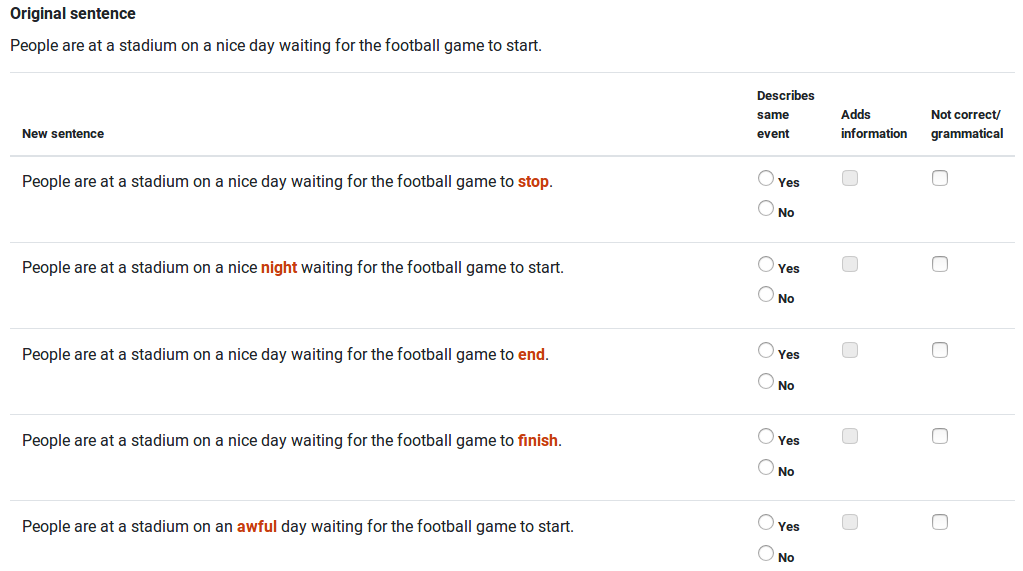
\includegraphics[totalheight=7cm]{fig/sample_hit.png}
	\caption{Example of a \ac{HIT} in Amazon Mechanical Turk.}
	\label{fig:example_hit}
\end{figure}
The questions are explained to the users with example \ac{HIT}s of the same form in the instructions. In order to make the task more attractive to annotators, without increasing the payment too much, we simplified the process by highlighting the exchanged words.
\newline

\noindent
We assign each \ac{HIT} to three annotators. After removing all invalid sentence-pairs, we consider the majority label as the gold label, if at least two annotators agree on it. Sentence-pairs without agreement are not considered for our new testset. After an inital annotation round of 1,000 samples, we remove categories and word-pairs, that show a high tendency of having invalid sentences. We show the statistics of our final testset, consisting of 8,193 sentence-pairs in Table \ref{tab:newtest_stats}.
\begin{table}[tph!]
\centering
\begin{tabular}{l|cccc|ccc}
& \multicolumn{4}{c}{\textbf{Instances}} & \multicolumn{3}{c}{\textbf{Fleiss $\kappa$}} \\
& contradiction & neutral & entailment & \textbf{Overall} & contradiction & entailment & \textbf{Overall} \\
\toprule
\textbf{SNLI Test}& 3,236 & 3,215 & 3,364 & \textbf{9,815} & 0.77 & 0.69 & \textbf{0.67} \\
\textbf{New Test}& 7,164 & 47 & 982 & \textbf{8,193} & 0.61 & 0.90 & \textbf{0.61} \\
\bottomrule
\end{tabular}
	\caption{Statistics of \ac{SNLI} testset compared with the newly generated testset.}
	\label{tab:newtest_stats}
\end{table}
As can be seen, the new test set is heavily focused on contradicting samples. Since this test set only serves, to measure the capabilities of a model in dealing with lexical inferences (and \ac{NLU} with reduced dataset-specific patterns), but not to replace the original \ac{SNLI} testset, this is not problematic. It still must be considered, when evaluating a model, as a simple baseline, predicting everything as contradiction, would result in an accuracy of 87.4\%. We report the agreement with Fleiss Kappa \citep{landis1977measurement} (over all samples and for the representative labels \textit{entailment} and \textit{contradiction}), as it was done by \cite{bowman2015large} for the original \ac{SNLI}. For better comparison, we re-calculate the numbers on all valid samples of the \ac{SNLI} testset. The new testset yields ``substantial agreement'' with a Fleiss Kappa of 0.61. It should be noted, that Kappa also considers, how likely a specific label would selected by chance, and for this purpose takes the overall label distribution into account. This does not influence the measure for the original \ac{SNLI}, since all labels are evenly distributed. For the new test set however, this method assumes that contradiction is more likely to appear by chance, due to its high frequency. As this results from our selected word-pairs rather than an underlying ``natural distribution'', the figure, calculated by Fleiss Kappa, might be less suited as an agreement measure for the new dataset. Yet, for very different reasons, it is indeed likely that annotators are slightly biased towards selecting contradiction, as the result of our \ac{HIT} presentation: Since most word-pairs are contradicting and word differences are highlighted, annotators might, to some extend, shift their focus more on the difference between those words, rather than solely on the actual word-usage in context. To provide an easier to interpret measure of this dataset, we estimate the human performance in the same manner, as done by \cite{gong2017natural} for \ac{SNLI}. They consider all samples with majoriy label, which results in the gold label, and calculate the ratio of annotator labels, matching the majority gold label, as the estimate for the human performance in terms of accuracy. Thus, let $g(x,y)$, with $x$ as the annotator label and $y$ as the estimated gold label, define, if the annotation counts as a misclassification or not:
\begin{equation}
g(x,y) = \begin{cases}
1 & \text{if $x = y$} \\
0 & \text{if $x \neq y$ }
\end{cases}
\end{equation}
Let furthermore $L$ contain all pairs $(x,y)$ of the annotated dataset and $|L|$ be the amount of elements within $L$. Following \cite{gong2017natural}, we estimate the human performance $a$ in accuracy as follows:
\begin{equation}
a = \frac{\sum_{(x,y) \in L} g(x,y)}{|L|}
\end{equation}
Doing so, we estimate the human performance on the new testset to be 94.1\%, slightly higher than the human performance estimated on \ac{SNLI} with only 87.7\%, indicating that our new sentence-pairs do not pose additional difficulties, but in fact indeed seem relatively easy for humans.
\subsection{Evaluation}
We evaluate three neural models without external knowledge other than the one from distributed word-embeddings, that achieve strong results on \ac{SNLI}. All models are retrained with different datasets, using the provided code and keeping all hyperparameters. We explain the experimental setup and results below. 
\subsubsection{Experimental setup}
\paragraph*{Models without external knowledge}
We evaluate the Residual-Stacked Encoder\textsuperscript{$\Diamond$} \citep{nie2017shortcut}, as explained in Section §\ref{sec:residual_encoder_def}, ESIM \citep{chen2017enhanced} and Decomposable Attention \citep{parikh2016decomposable}, both explained in Section §\ref{sec:models_snli}. The published model of ESIM ensembles two models with different sentence encoding strategies, one is based on a TreeLSTM, the other on a \ac{biLSTM}. For our experiments we retrain only the \ac{biLSTM}-based model. For Decomposable-Attention, we use the AllenNLP re-implementation\footnote{\href{http://allennlp.org/models}{http://allennlp.org/models}}. As opposed to the reported version on the SNLI leaderboard\footnote{\href{https://nlp.stanford.edu/projects/snli/}{https://nlp.stanford.edu/projects/snli/}} this implementation does not use the optional intra-sentence attention. Its performance on the \ac{SNLI} test is with 84.7\% slightly lower, but comparable to the model with intra-sentence attention (86.3\%). All models have different characteristics, depticted in Table \ref{tab:compare_architecture_models} and are at the time of the experiment amongst the best within their categories.
\begin{table}[tph!]
\centering
\begin{tabular}{r|ccc}
& \specialcellc{\textbf{Finetune}\\\textbf{Embeddings}} & \textbf{LSTM-based} & \specialcellc{\textbf{Inter-sentence}\\\textbf{Attention}} \\
\toprule
Decomposable Attention \citep{parikh2016decomposable} & $-$ & $-$ & \textit{yes}\\
Residual-Stacked Encoder \cite{nie2017shortcut} &\textit{yes}  &\textit{yes} & $-$\\
ESIM \citep{chen2017enhanced} &\textit{yes} &\textit{yes} & \textit{yes}\\
\bottomrule
\end{tabular}
\caption{Architectural comparison of tested neural models without external knowledge.}
\label{tab:compare_architecture_models}
\end{table}

\subsubsection{Models with external knowledge}
Additionally we also provide a simple WordNet baseline, predicting the relationship of ($p$,$h$) by assuming all sentences to be upward-monotone and, thus having the same relation as ($w_p$,$w_h$). Specifically, for each ($w_p$,$w_h$) we check their lexical semantic relation within WordNet, and map it to a relation label in the following manner:
\begin{itemize}
\item \textbf{Synonymy:} Synonyms are predicted as \textit{entailment}.
\item \textbf{Antonomy:} Antonyms are predicted as \textit{contradiction}.
\item \textbf{Hypernomy:} If $w_p$ is a hypernym of $w_h$ the sentence-pair is predicted as \textit{neutral}, if $w_p$ is a hyponym of $w_h$ as \textit{entailment}.
\item \textbf{Co-hyponomy:} Cohyponyms are predicted as \textit{contradiction}. We only only consider co-hyponyms with a maximum distance of two edges in the ontology to their common hypernym, as considering all potential co-hyponyms would yield all ($w_p$,$w_h$) coming from the same (very general) root-word to be labelled as contradiction.
\end{itemize}
We map multi-word expressions like ``at night'' to their meaning-carrying word (``night''), if the function words have only been added for a higher precision, when replacing the words in the generation process. In case they refer to actual entities (e.g. ``New Zealand''), we identify the applicable synsets of the whole expression in WordNet. As explained in Section §\ref{sec:wordnet}, words may have several synsets leading to potentially several different lexical relations amongst the words of interest $w_p$ and $w_h$. For each relation between both words, we calculate a score $s=\max(r_p,r_h)$ with $r_p$ and $r_h$ being the rank of the synset of the word $w_p$ and $w_h$ respectively. This follows the common heuristic that dominant senses appear as the first synsets while rare senses appear at the end \citep{mccarthy2004using}. Subsequently, if several lexical relations exist, we consider the one with the lowest assigned score as tie-breaker\footnote{In case the score $s$ is identical for several relations, we select the relation in the following order ($X > Y$ meaning $X$ is preferred over $Y$):\\ synonym $>$ antonym $>$ hypernym $>$ hyponym $>$ co-hyponym } and thus, tend to focus on more dominant word-senses. Of course, this baseline only is possible, if knowing that $p$ and $h$ only differ in $w_p$ and $w_h$ and is thus not applicable to sentence-pairs in general. Yet it provides insight, to what extend information within WordNet can help on our new test set. In addition to that we, also report\footnote{We did not conduct the experiment with \ac{KIM} ourselves, but received their results from the orignal authors recently. The analysis part thus does not contain deeper analysis of the performance of KIM.} the results of \ac{KIM} \citep{chen2017natural}, as explained in Section §\ref{sec:rel_work_sentence_encoding_models}.
\paragraph*{Traing data}
In addtion to training all models on \ac{SNLI}, wich is considered relatively easy, we also train each model on the union of SNLI and \ac{MultiNLI} and SciTail respectively, both are assumed to be more difficult and explained in deeper detail in Section §\ref{sec:basics_datasets}. The motivation is, that while SNLI might lack the training data needed, to learn the required lexical knowledge, this data may be available in the other datasets, which are presumably less simple. 
\subsubsection{Results}
The results for each model with the according train sets are visualized in Table \ref{tab:adv_results}.
\begin{table}[tph!]
\centering
\begin{tabular}{c c c c c c}
\toprule
\textbf{Model} & \textbf{Train set} & \textbf{SNLI test set} & \textbf{New test set} & $\Delta$ \\ 
\midrule
\multirow{3}{*}{\specialcellc{Decomposable Attention \\ \citep{parikh2016decomposable}}} & SNLI & 84.7\% & 51.9\% & -32.8 \\ 
& MultiNLI + SNLI & 84.9\% & 65.8\% & -19.1 \\ 
& SciTail + SNLI & 85.0\% & 49.0\% & -36.0 \\ 
\midrule
\multirow{3}{*}{\specialcellc{ESIM \\ \citep{chen2017enhanced}}} & SNLI & 87.9\% & 65.6\%& -22.3\\ 
& MultiNLI + SNLI & 86.3\% &74.9\% & -11.4\\
& SciTail + SNLI & 88.3\% & 67.7\%& -20.6\\ 
\midrule
\multirow{3}{*}{\specialcellc{Residual-Stacked Encoder\textsuperscript{$\Diamond$} \\ \citep{nie2017shortcut}}} & SNLI & 86.0\% & 62.2\% & -23.8\\ 
& MultiNLI + SNLI & 84.6\% & 68.2\%& -16.8\\ 
& SciTail + SNLI & 85.0\% & 60.1\%& -24.9\\ 
\midrule
WordNet Baseline & - & - & 85.8\% & - \\ 
KIM \citep{chen2017natural} & SNLI & 88.6\% & 83.5\% & -5.1 \\ 
\bottomrule
\end{tabular}
\caption{Results of models on the new test set compared with the original \ac{SNLI} test set.}
\label{tab:adv_results}
\end{table}
There is a clear trend, that adding \ac{MultiNLI} to the training data boosts the model's performance on the new test set. At the same time it decreases the test accuracy on SNLI, indicating that the performance, gained on \ac{SNLI} test, does not reflect the true \ac{NLU} capabilities, since clearly less lexical semantic relations are understood. Yet, compared with the original estimated performance, even by almost doubling the amount of train data with \ac{MultiNLI}, all models without external knowledge show a significant drop in performance. While MultiNLI follows the same labelling scheme as SNLI, and thus is compatible, SciTail does not specifically assume event coeference and lacks having the label \textit{contradiction}, which is dominant in the new test set. Hence, the models seem to not be able to leverage from the extended amount of data in this case. Both models with WordNet information perform significantly better than the ones without. This shows, that the lexical relations, as contained in WordNet, are sufficient to gain strong improvements on the new dataset. In addition to that, those relations have also shown to be useful for \ac{KIM} in training on \ac{SNLI} (as they are considered for the prediction). This especially shows some crucial drawbacks in the neural models without WordNet, as they clearly lack to extract those features when trained solely with textual input, by learning features based on arbitrary patterns at the cost of also meaningful (for \ac{SNLI} and naturally for \ac{NLU}) features of lexical relations. Only dropping by 5.1 points in accuracy w.r.t. the performance on \ac{SNLI}, \ac{KIM} seems substentially more stable, when sentences are adapted, forcing the model to predict based on a language understanding rather than dataset specific patterns. This of course may be due to the fact, that the new testset, being closely related to the train data and requiring the same knowledge, as added for \ac{KIM}, is highly suitable for\ac{KIM}. Thus, it still does not prove truely superior \ac{NLU}, yet it shows that they found a successful strategy of integrating this resource into neural models.

\subsection{Analysis}
We take a closer look on the performance achieved by the models without external knowledge. As the performance only improves marginally, if the train data is tremendously increased by adding \ac{MultiNLI}, we focus our analysis part on the models, solely trained on the original \ac{SNLI} dataset.
\subsubsection{Accuracy by category}
Table \ref{tab:acc_by_cat} shows the accuracy per category, as defined when creating the word-pairs, for all models, including \ac{KIM} and the WordNet baseline. As not all categories contain an even amont of sanples, we additionally supply information about this figure, together with sample words for a better understanding, what each category represents. Originating from our word-pairs, almost all categories are majority labelled contradiction, solely synonyms mostly are labelled as entailment.
\begin{table}[tph!]
\centering
\begin{tabular}{lrc|ccccc} 
\toprule
\textbf{Category} & \textbf{Amount} & \specialcellc{\textbf{Example}\\\textbf{Words}} & \specialcellc{\textbf{Decomposable}\\\textbf{Attention}} & \textbf{ESIM} & \specialcellc{\textbf{Residual}\\\textbf{Encoders}} & \specialcellc{\textbf{WordNet}\\\textbf{Baseline}} & \textbf{KIM}  \\ \midrule
antonyms & 1,147 & \textit{loves - dislikes} & 41.6\% & 70.4\%& 58.2\% &  95.5\% & 86.5\% \\ 
cardinals & 759 &\textit{five - seven} & 53.5\% &75.5\% & 53.1\% & 98.6\% & 93.4\% \\ 
nationalities & 755 & \textit{Greek - Italian} & 37.5\% &35.9\% & 70.9\% & 78.5\% & 73.5\% \\ 
drinks & 731 & \textit{lemonade - beer} & 52.9\% &63.7\% & 52.0\% & 94.8\% & 96.6\% \\ 
antonyms (WN) & 706 & \textit{sitting - standing} & 55.1\% & 74.6\%& 67.9\% & 94.5\% & 78.8\% \\
colors & 699 & \textit{red - blue} & 85.0\% &96.1\% & 87.0\% & 98.7\% & 98.3\% \\ 
ordinals & 663 & \textit{fifth - 16th} & 2.1\% &21.0\% & 5.4\% &40.7\% & 56.6\% \\ 
countries & 613 & \textit{Mexico - Peru} & 15.2\% &25.4\% & 66.2\% & 100.0\% & 70.8\% \\ 
rooms & 595 & \textit{kitchen - bathroom} & 59.2\% &69.4\% & 63.4\% & 89.9\% & 77.6\% \\ 
materials & 397 & \textit{stone - glass} & 65.2\% & 89.7\%& 79.9\% & 75.3\% & 98.7\% \\
vegetables & 109 & \textit{tomato -potato} & 43.1\% &31.2\% & 37.6\% & 86.2\% & 79.8\% \\ 
instruments & 65 & \textit{harmonica - harp} & 96.9\% &90.8\% & 96.9\% & 67.7\% & 96.9\% \\ 
planets & 60 & \textit{Mars - Venus} & 31.7\% & 3.3\%& 21.7\% & 100.0\% & 5.0\% \\ 
\midrule
synonyms & 894 & \textit{happy - joyful} & 97.5\% & 99.7\% & 86.1\% & 70.5\% & 92.1\% \\ 
\midrule
total & 8,193 &  & 51.9\% &65.6\% & 62.2\% & 85.8\% & 83.5\% \\ 
\bottomrule
\end{tabular}
\caption{Accuracy reached for the tested models for each category with assoziated sample words and the amount of instances.}
\label{tab:acc_by_cat}
\end{table}
All neural models achieve good results on categories that occur very frequently within \ac{SNLI} in general, like \textit{colors}. Also \textit{instruments} are well captures. We find that muscic instruments often occur in SNLI in very similar sentences containing some kind of \texttt{actor} and in conjunction with the instrument and the verbs "hold" or especially "play". In contradicting samples of the train data, in most cases the instrument changes. Thus our newly created sentence-pairs are very similar to those within the train data, explaining the good performance within that category. On the other hand, categories that are rare in \ac{SNLI}, like \textit{planets} or \textit{ordinals}, are not well understood by those models. As opposed to to \textit{instruments}, the relevance of \textit{ordinals} within a sentence in \ac{SNLI} usually is less crucial. Yet this originates only the commonly applied strategies by the annotators, as identified by \cite{gururangan2018annotation}. Consider for instance the sentence ``"A man racing his motorcycle comes in \textit{first}."'', which naturally yields in contradiction if we replace ``first'' by ``eights''. Yet the model without external information seemingly do not differentitate between both ordinal numbers, as annotators rather tend to change ``man'' or even ``motorcycle'', but not ``first''. Also \textit{drinks}, \textit{vegetables} and \textit{rooms} are generally harder for the model to predict for similar reasons. The reason for \textit{antonyms} being more difficult  than \textit{antonyms\_WordNet} most like arises from the fact, that they include gender-related antonyms, appearing in SNLI in abundance, that we do not include within the hand-crafted word pairs. As \textit{synonym} examples have large lexical overlap and differ only by one word, occuring in similar contexts (and subsequentially having a similar word-vector), it is no surprise, that all models achieve a good performance here. Inter-sentence-attention seems to have an advantage in this case, since only the Residual-Stacked Encoders does not improve significantly over its original test performance. We thus focus the remaining part of the analysis on contradicting sentence-pairs only.

\subsubsection{Impact on the word embeddings}
As previously pointed out, word-pairs with the lexical semantic relations, antonymy and co-hyponynomy, in many cases result in similar word representations with distributed embeddings. Subsequentially, we first analyse the impact of those word-representations, leveraging from the fact, that sentence-pairs in our new dataset only differs in one known word.
\paragraph*{Without fine-tuned embeddings}
Figure \ref{fig:decomp_acc_per_cos_sim} visualizes the performance of all contradicing samples, compared to the cosine similarity between the word-vectors of $w_p$ and $w_h$, achieved by Decomposable Attention. 
\begin{figure}[tph!]
\centering
	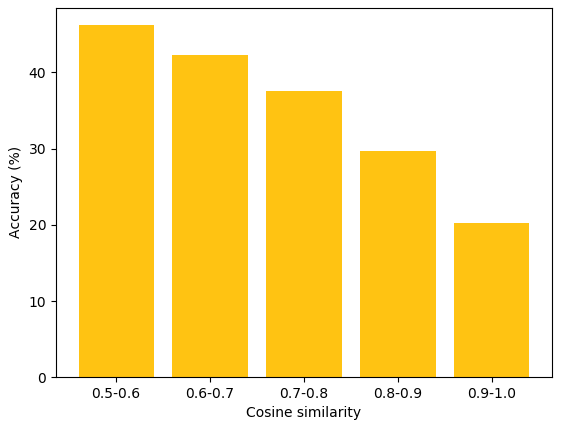
\includegraphics[totalheight=5cm]{fig/acc_by_cos.png}
	\caption{Accuracy by cosine similarity reached by Decomposable Attention (without fine-tuned embeddings).}
	\label{fig:decomp_acc_per_cos_sim}
\end{figure}
We exclude any multi-word expressions in this analysis. Let $v_p$ and $v_h$ be the word vectors of the GloVe embeddings, used by Decomposable Attention, the according cosine simmilarity $\cos(v_p,v_h)$ is calculated as follows:
\begin{equation}
\cos(v_p,v_h) = \frac{v_p v_h}{|v_p| |v_h|}
\end{equation}
We observe, that without fine-tuned embeddings, the reached accuracy highly correlates with the similarity of the word representations even though Decomposable Attention uses only the lower-cased word embeddings and thus contains comparably more samples per word-vector than the other two models, ESIM and Residual-Stacked Encoder. Those models rely on cased word-embeddings, and we could not find the same correlation between the accuracy and word-similarity. We assume this stems from the fact, that both models fine-tune embeddings and thus push contradicting words, as seen in the training, further apart in the embedding space. 
\paragraph*{With fine-tuned embeddings}
We evaluate the accuracy of both models with fine-tuned embeddings w.r.t. the amount $w_p$ and $w_h$ seen during training on \ac{SNLI} and visualize the results in Figure \ref{fig:esim_res_acc_by_freq}.
\begin{figure}[tph!]
\centering
	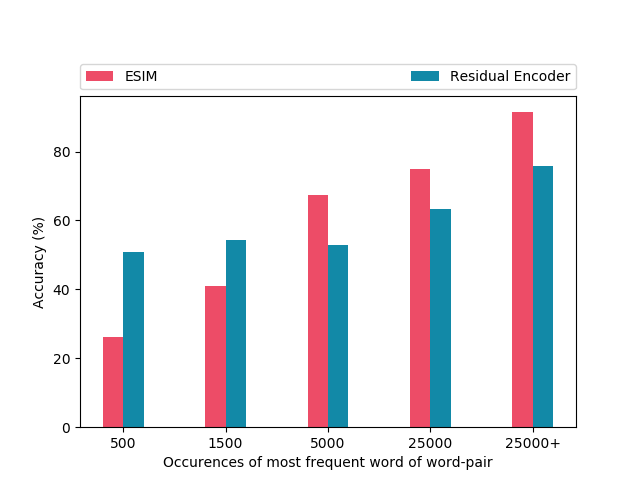
\includegraphics[totalheight=6cm]{fig/esim_res_acc_by_freq.png}
	\caption{Accuracy by word freqency for Residual-Stacked Encoder and ESIM.}
	\label{fig:esim_res_acc_by_freq}
\end{figure}
The numbers on the x-axis show the upper bound of word occurences of the word-pair, denoted as $a_{(w_p,w_h)}$, responsible for creating each sentence-pair. Specifically, we calculate the $a_{(w_p,w_h)}$ by taking the more frequent word within \ac{SNLI} train data, thus $a_{(w_p,w_h)} = \max(a_{w_p},a_{w_h})$, with $a_{w_p}$ and $a_{w_h}$ being the amount of sentences, containing $w_p$ and $w_h$ respectively. In case, one of $w_p$ or $w_h$ is an expression containing multiple words, denoted as $e = [w_1, \ldots , w_{n-1}, w_{n}]$, we calculate the according amount, denoted as $a_e$, by considering the least frequent word: $a_e = \min(w_1, \ldots , w_{n-1}, w_n)$. Intuitively, this will ignore added function words and, in most cases, focus on the meaning-carrying word within the expression. Both models depend on the same underlying GloVe word-embeddings, yet it seems that Residual-Stacked Encoder\textsuperscript{$\Diamond$} achieves better results on less frequent words.  While still performing considerably worse with fewer examples seen, the more individually created sentence representations, as trained in this model, generalize better for sparcely present lexical relations. As opposed to the Residual-Stacked Encoder, ESIM seems to heavily depends on a high frequency of the words to classify sentence-pairs correctly.  While ESIM performs very poor for less frequent words, it shows to quickly increase in performance with an increasing amount of samples, containing the same words, within the train data. This presumeably arises from the inter-sentence attention, aligning words from both sentences with each other. The resulting sentence representations are therefore less general and suited for the individual word relations of both sentences, leading to a higher performance, if similar word relations have previously been seen in training; at the same time however, reducing the generalization capabilites. Subsequentially we take a closer look into the performance of ESIM, the best of all three evaluated neural models without external knowledge, and compare the amount of similar samples seen during training with the reached accuracy. We count samples ($p$, $h$) from the train data with the gold label contradiction and consider them, if they contain $w_p$ in $p$ and $w_h$ in $h$, \textit{similar} to all samples in the new dataset, arising from ($w_p$,$w_h$). 
\begin{table}[tph!]
\centering
\begin{tabular}{l|c|c|c|c|c|c}
\toprule
\textbf{Frequency} & 0 & 1 -- 4 & 5 -- 9 & 10 -- 49 & 50 -- 99 & 100+ \\
\midrule
\textbf{Accuracy} & 40.2\% & 70.6\% & 91.4\% & 92.1\% & 97.5\% & 98.5\% \\
\bottomrule
\end{tabular}
\caption{Accuracy by the amount of similar samples in \ac{SNLI} train data for ESIM on contradicting samples.}
\label{tab:esim_acc_by_sim_samples}
\end{table}
The results are shown in Table \ref{tab:esim_acc_by_sim_samples}.
It can be seen, that indeed, the performance of \ac{ESIM} is high, if it has seen $w_p$ and $w_h$ in a contradicting context in a sufficiently high amount, whereas it performs poorly, if it has not seen both words within a contradiction-labelled sample at least once. This shows, that the comparably higher performance of ESIM is matter of memorizing ($w_p$,$w_h$) as being contradictive, rather than generalization over similar constructs. Similarily, this explains the increase in accuracy when adding \ac{MultiNLI}, not because it learns to generalize better, but because it has seen slightly more contradictive word-pairs in a contradicting context. While this is sufficient to achieve a high performance on \ac{SNLI}, we show that the main goal of machine learning, to generalize over unseen textual constructions, in this case is not met. 

\subsection{Conclusion of the adversarial dataset}
We show that state-of-the-art NLI systems with only pretrained word embeddings as external information trained on any of these datasets are limited in their generalization ability and fail to capture simple inferences. Additionally, we show, that the SNLI test set alone is not a sufficient measure of the languge understanding capabilities of a model, using our newly created test set. As the high performance arises from arbitrary patterns, that we excluded in our dataset, this number is in fact somewhat misleading, considering that \ac{NLI} originally is meant to be closely related to \ac{NLU} capabilites of the models \citep{williams2017broad}. While models without external knowledge perform good by memorizing patterns, the relevant information for the new testset are also useful for \ac{SNLI} and improve the model's generalization abilities. Both knowledge-rich approaches achieve comparably high performances on the new dataset, but still have a potential for improvement. Those may either be tackled by a resource with a higher coverage than WordNet, or by improving lexical inference in context \citep{shwartz2016adding}.